\newglossaryentry{md5}{name=MD5, description={The MD5 algorithm is a widely used hash function producing a 128-bit hash value}}
\newglossaryentry{cpu}{name=CPU, description={Central processing unit}}
\newglossaryentry{os}{name=OS, description={Operating system}}
\newglossaryentry{gpu}{name=GPU, description={Graphical processing unit}}
\newglossaryentry{ram}{name=RAM, description={Random-access memory}}


\chapter{Experiments} % Write in your own chapter title
\label{chap:experiments}
\lhead{Chapter 5. \emph{Experiments}} % Write in your own chapter title to set the page header

In this section different type of experiments are conducted in order to test and check the performance of the developed software.

\section{Test script and machine}
In order to conduct the different experiments, we chose a test script available online on \textit{TheAlgorithms} \href{https://github.com/TheAlgorithms/Python/blob/master/hashes/md5.py}{GitHub page}. We selected this test script because \gls{md5} checking is a really common task and generates many numerical values for which our solution is the most intended. 

Concerning the testing machine itself, we chose to run the tests directly on our personal laptop because it correspond to the usage the system is intended for : a personal debugging tool. The specifications of the machine are the following ones :
\begin{itemize}
  \item Lenovo Thinkpad T460p
  \item \gls{cpu} : Intel Core i7-6700HQ @ 2.60GHz x 8
  \item \gls{os} : Fedora 25 64bits
  \item \gls{gpu} : Intel HD Graphics 530
  \item \gls{ram} : 15.1Gio
\end{itemize}

\section{Objectives}
For the experiments, we want here to test two aspects of our system : the memory usage and the runtime. To be able to measure these two parameters, we use a Python tool called \textit{Memory profiler}. This tool is for monitoring memory consumption of a process as well as line-by-line analysis of memory consumption for python programs. It allows also to plot memory consumption as a function of time and measure the execution time of the target script. With these extracted parameters, the tool is also capable to plot graphs. Our aim is to verify if dynamic analysis induces overhead with the help of the memory profiler and our dynamic analysis solution.

\section{Performances}
\subsection{Test script}
The first necessary step in order to conduct our experiments correctly, is to create a reference run from which we will be able to compare our results.
In this idea, we profiled the memory consumption and the runtime of the test script without plugging in our system. The \autoref{fig:memumd5} illustrates the results of the Memory profiler: the test script uses a total of 13.45MiB of memory for a runtime of 0.1s.
\begin{figure}[h!]
  \centering
    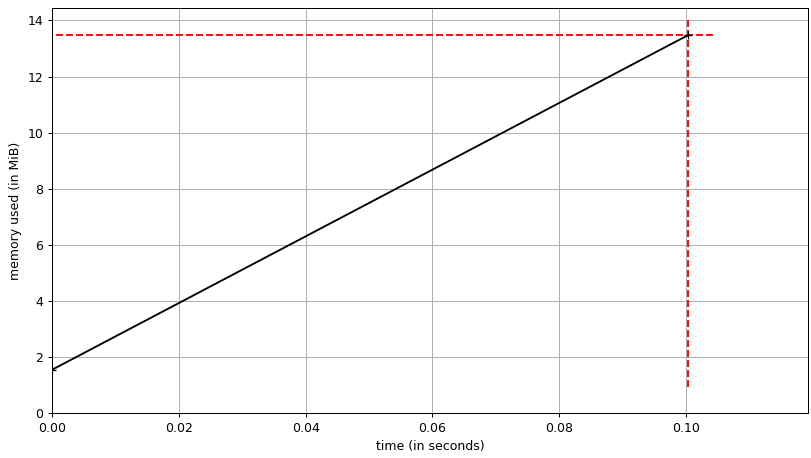
\includegraphics[width=\textwidth]{figures/experiments_figure_md5.png}
    \caption{Memory usage and runtime of the test script}
    \label{fig:memumd5}
\end{figure}
\subsection{Data capture}
The first process in our solution which could induce overhead is the data capture process and therefore, we want here to test its performance. In order to exclusively determine the memory usage and runtime of the data capture process, we activated the debug mode of the system to avoid the database writing process. 

The \autoref{fig:memuyoda} presents the results of the memory profiler analysis. As we supposed, the process is inducing overhead. The execution time is now of 0.6s which represents a multiplication by 6 compared to the reference test. Concerning the memory the script now needs 27.6MiB of RAM which is more than the double of the original run.
\begin{figure}[h!]
  \centering
    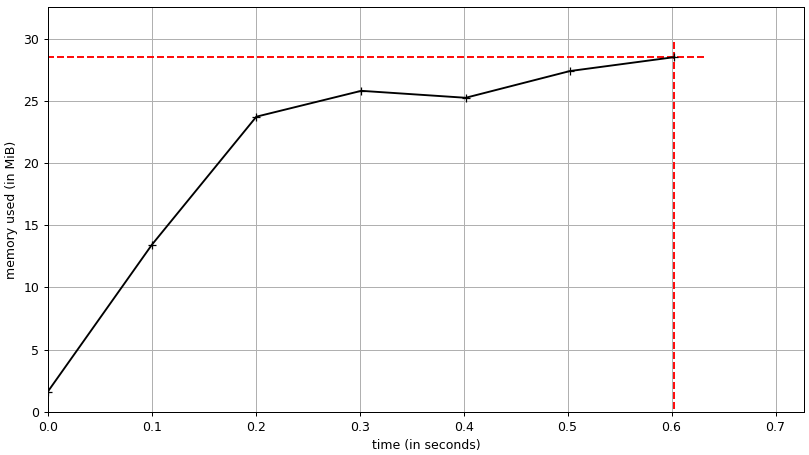
\includegraphics[width=\textwidth]{figures/experiments_figure_yoda.png}
    \caption{Memory usage and runtime with the Yoda system activated}
    \label{fig:memuyoda}
\end{figure}

These results could be seen as deceiving but in fact are inevitable because of the nature of our solution. Indeed, because we want to track the value of each variable at each line, the values are not overridden as in the normal run of the script. Instead, for each value, we store in the memory a copy of the variable and its data.

\subsection{Database writing}
The second process of interest which we want to test here is the database writing process. By activating this phase in the tool, we want to see if it also induces an overhead. 

As it is shown in the \autoref{fig:memudb}, the introduction of the data writing process in our test does not induce any significant extra memory usage which is now at the maximum around 29MiB. Nonetheless, the writing process induce a runtime overhead of 0.5s to now reach a total of 1.21s.
\begin{figure}[h!]
  \centering
    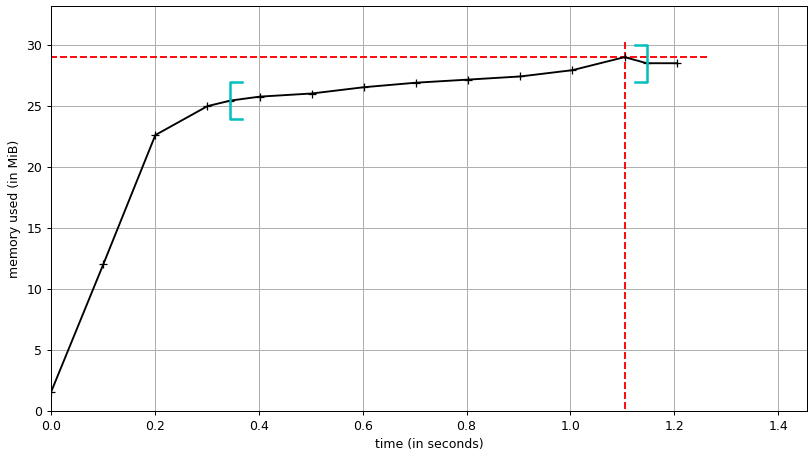
\includegraphics[width=\textwidth]{figures/experiments_figure_db.png}
    \caption{Memory usage and runtime with the database writing}
    \label{fig:memudb}
\end{figure}

\section{Concluding remarks}

In the \autoref{chap:relatedwork}, we already introduced some limitation of dynamic analysis tools, which is often heavy runtime overhead. We showed in the experiments that our solution is not an exception and induces even on a small script a heavier memory consumption and a significant runtime overhead. An idea to optimize the process could be asynchronously writing via a message queue.

It has to be pointed out that the memory profiler is not an exact tool. Indeed, according to \cite{Pedregos2016}, this module gets the memory consumption by querying the operating system kernel about the amount of memory the current process has allocated, which might be slightly different from the amount of memory that is actually used by the Python interpreter. Also, because of how the garbage collector works in Python the result might be different between platforms and even between runs.
